\documentclass[letterpaper,10pt]{article}

%\setlength{\parindent}{0in}
%\usepackage{fullpage} 
\usepackage{amsmath}
\usepackage{amssymb}
\usepackage{enumerate}
\usepackage{graphicx}
\usepackage[table]{xcolor}
\usepackage{dcolumn}
\oddsidemargin 0.0in
\textwidth 6.5in
\newcolumntype{.}{D{.}{.}{-1}}
\newcommand*{\myalign}[2]{\multicolumn{1}{#1}{#2}}
\usepackage{lastpage} % for the number of the last page in the document
\usepackage{fancyhdr}
\pagestyle{fancy}
\fancyhf{}
\lfoot{Lab Group 6: Case Study}
\rfoot{Page \thepage\ of \pageref{LastPage}}

%opening
\title{Case Study}
\author{Lab Group 6 \\ { \small (Steve Mazza, George Palafox, Donna Ray)}}
\date{April 25, 2012}

\begin{document}
\maketitle

\section{The Problem}
Mohawk, large bank that had operated with a traditional management structure for over a decade, decided that it needed to consider a matrix structure in order to help overcome some bureaucratic problems caused by recent growth.  According to the case study background, ``The traditional organization was too weak structurally to handle problems that required integration across multiple departments.''\footnote{Kerzner, \emph{Project Management Case Studies} (New York: Wiley \& Sons, 2009) pp 232.}

The decision was made to pursue a matrix structure and several difficulties resulted.  First, there was some hesitation from top management.  Acknowledging the need for talented project management from the start, Pat Coleman, Vice President for Operations, commented, ``I'm still not sure whether we should promote from within or hire from outside.''\footnote{Ibid, pp 233.}  Nonetheless, he asked the Director of Personnel, Randy Gardner, to identify the four most promotable candidates from within the organization.

Two weeks later Randy Gardner reported back that none of the intended candidates would immediately take the position.  The dilemma remained: look for additional internal employees or look externally.

\section{Considerations}
\subsection{Question 1}
\emph{How do you implement change in a bank?}\vspace*{1em}\vspace*{1em}

Since the banks tend to follow traditionalism and regimentation, basically do what works already, it will be very hard to implement change within the bank.  As Randy Gardner, the director of personnel explains, department managers will not have a problem adopting; it will be the functional employees that will resist change.  Furthermore, Mr. Gardner explains that functional employees won't accept change until they see the new form of organization work.  Therefore, in order to implement change, a good solid plan must be set in place and quickly be ready to execute to implement this new type of organization.  The slightest mistake or inkling that things are not going according to plan will cause employees to resist to change and it will take a while before another attempt can be entertained.  It also appears that some top key performers, based on what Mr. Gardner's report to Mr. Coleman states, don't want to engage in becoming a Project Manager (PM).  One employee was up for the challenge but felt he was too inexperienced and would fail.  I think it is always a good idea to promote within if possible.  This sends a strong message to the workforce with regards to opportunities and upward mobility in the ladder of success.  Perhaps as part of the implementation both alternatives can be used where some experienced managers would be hired from outside and more training could be provided to those that have a strong desire to become program managers.  

\subsection{Question 2}
\emph{What are some of the major reasons why employees do not want to become project managers?}\vspace*{1em}

Some of the reasons the employees don't want to become project managers include the following.
\begin{itemize}
\item Doesn't want to change in career fields.
\item Loss of established work relationships with co workers.
\item Not believing in the applications of Project Management
\end{itemize}

\subsection{Question 3}
\emph{Should the first group of project managers be laterally assigned?}\vspace*{1em}

I think that it would be a great idea to get some department managers trained and get some experience in the areas of project management to see the value it would add to the organization.  The article states that some managers don't fully embrace the concept of PM and it would be a great idea if they got some exposure to PM so that they can see the value added.  Since this would be a 6-month assignment, it would only be temporary so if the department manager desired to not continue then they would be returned to their original duty.

\subsection{Question 4}
\emph{Should the need for project management first be identified from within the organization?}\vspace*{1em}

Absolutely, since many folks are reluctant to embrace change, it would important to show why project management is needed within the organization and how the current processes will become more efficient and effective as a result of adopting PM.  If a strong need is identified, then functional employees will be more willing to embrace PM.

\subsection{Question 5}
\emph{Can project management be forced upon an organization?}\vspace*{1em}

PM cannot be forced upon an organization, but it can be coerced.  Management can decide that PM is the way forward, and devise planning and structure and deploy the execution.  Eventually the project has to be accepted by the functional staff and management has to deal with the development of relationships with staff organizations.  These relationships have to be developed in accordance with the organization of the functional teams and it matters that the PM understands and works with the functional management.

PM have to set the stage with the functional managers so that functional employees feel good about the change and set up functional employee (staff) training and feedback.  Lean Six Sigma is one possible good method of adapting the existing organization to project management.  These functional employees know their jobs and their roles and they will be instrumental in evolving the organization.  Each department is working independently and from the top of the organization, Mohawk Bank is starting at a point of virtual chaos, so going to a company-wide matrix organization solution is important to get the organization back on track quickly.

\subsection{Question 6}
\emph{Does the bank appear to understand project management?}\vspace*{1em}

The bank seems to have a partial understanding of PM.  The VP understands that good communication channels between the PM and functional management are needed.  The VP's notion of the organization structure has the PMs reporting to himself but he believes that the functional managers will be unhappy as a support group for the PM.  This notion does not include the concept that the functional employees are the working staff of the PM and that the functional management is part of that organizational alignment.  

\begin{center}
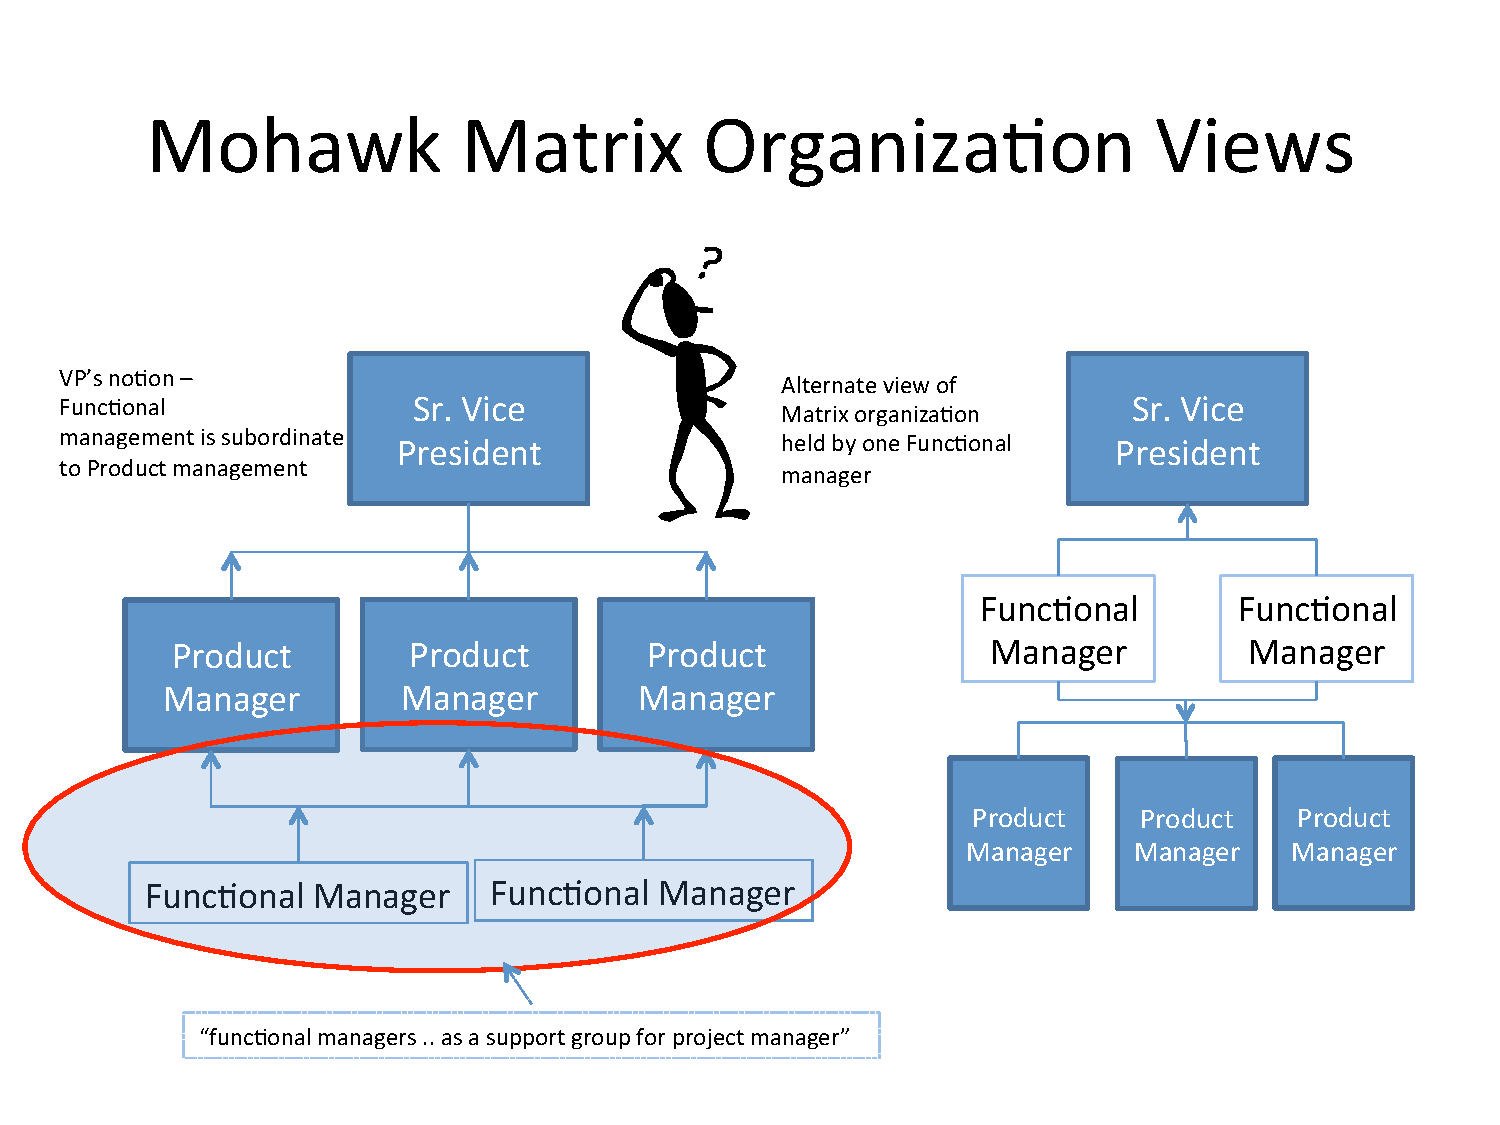
\includegraphics[scale=0.35]{figure1.pdf}
\end{center}

Mohawk VP's notion of matrix organization is that the functional managers are a support group for the product managers and he believes the functional managers will be unhappy in this role.  His vision is seems more like a traditional hierarchal organizational structure.  There is not a unity of opinion at Mohawk about the structure of the matrix organization, evidenced by an alternate view of power structure of the matrix organization from one of the candidates for Product manager. He had a vision of the organization that placed the functional management, (at least for his position in commercial loans) above the Product management position. 

\begin{center}
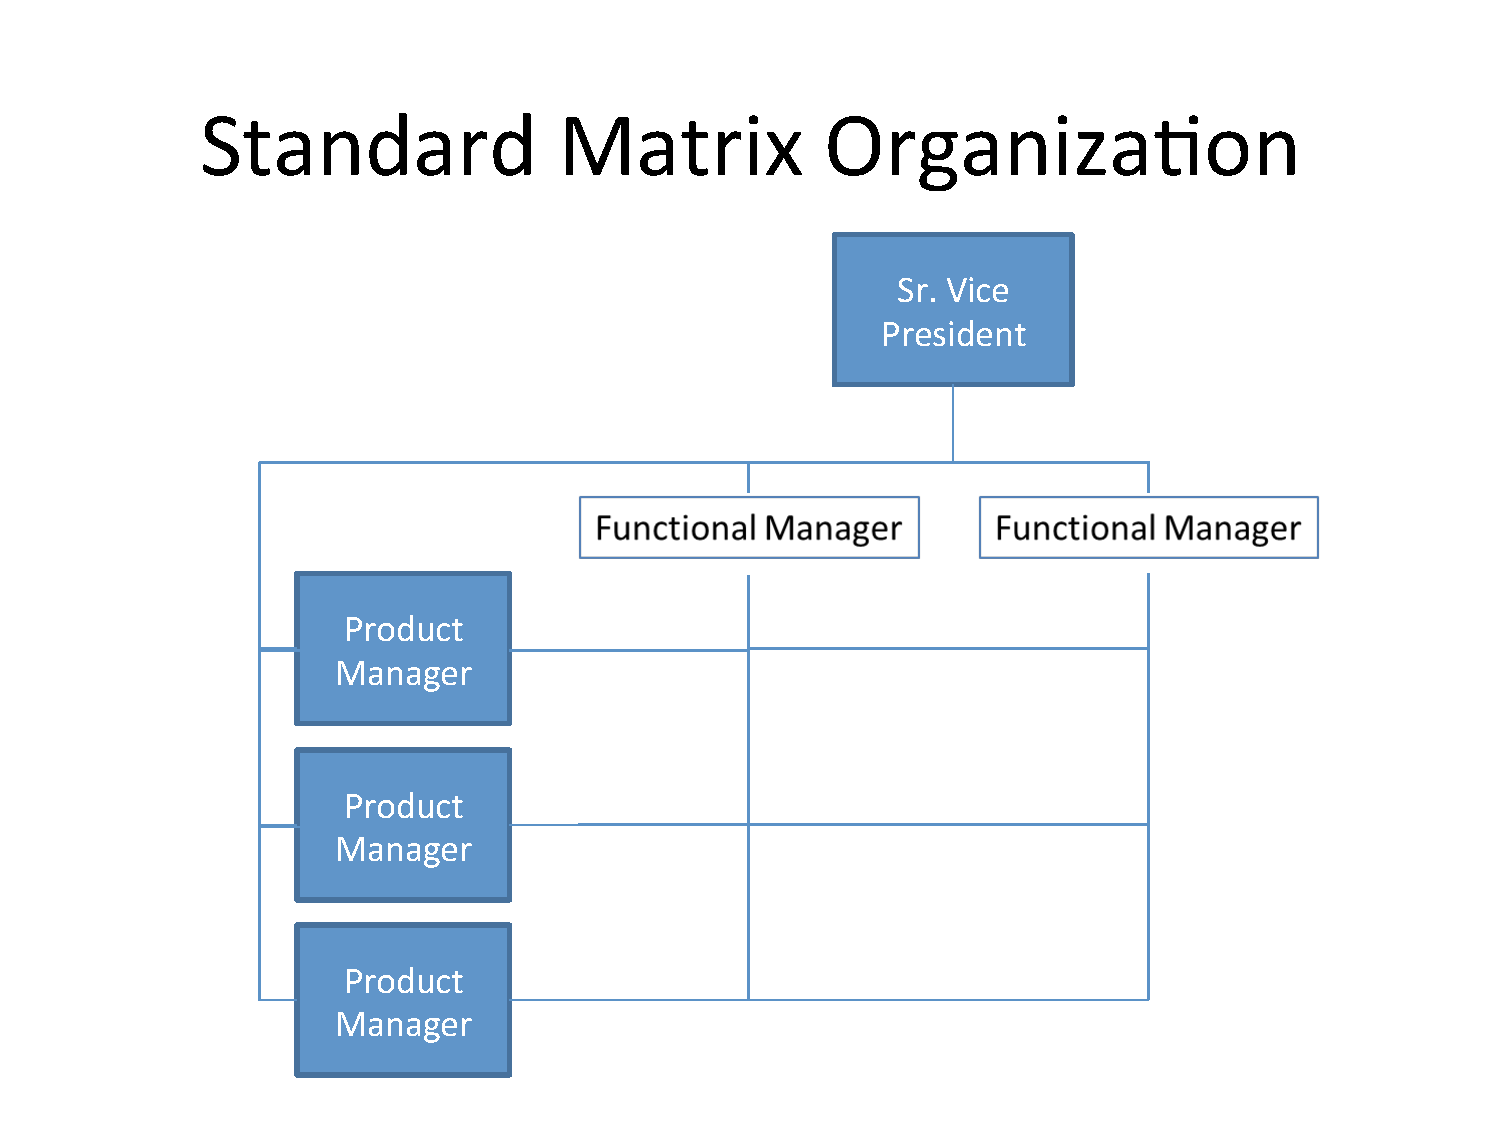
\includegraphics[scale=0.35]{figure2.pdf}
\end{center}

In a true matrix organization, the functional management and the product management are organized in a matrix.  This is a different management structure than the hierarchal organization represented by the views of the VP and the commercial loans functional manager.

\subsection{Question 7}
\emph{Should you start out with permanent or temporary project management position?}\vspace*{1em}

If the PM slot is temporary, and as the Bank VP suggested a six month trial is used to decide if the PM will be permanently assigned or rolled back to his or her functional position, then the probationary PM will be cautious and wary during the critical period for formation of team alliances.  Knowing that the PM will be permanent gives the staff a greater stake in establishing relationships with the PM that will be mutually beneficial. 

\subsection{Question 8}
\emph{Should the first group of project managers be found from within the organization?}\vspace*{1em}

The first set of PMs should be selected from outside the organization.  All the candidates for PM for the PM slots had reservations or negative feelings about taking the job of PM.  Although the insiders have an intimate familiarity with the current organization, that is part of the problem.  They are individualistic and will try to impose their functional views on the project wide management.  

\subsection{Question 9}
\emph{Will people be inclined to support the matrix if they see that the project managers are promoted from within?}\vspace*{1em}

Very junior people in the organization might be inclined to support the organization if they see that people are promoted from within, but more seasoned employees could see it as competitive situation with negative results for forming strong intra-team alliances with other staff members.

Overall support for matrix organization may be higher, however, if employees recognize the commitment from their peers and current management.  If positions are filled from within the organization then the readjustment should be somewhat eased due to a) the perception of support from within, and b) the ability to leverage existing relationships in the new organization.

\subsection{Question 10}
\emph{Suppose that the bank goes to a matrix, but without the support of top management.  Will the system fail?}\vspace*{1em}

While the system is not guaranteed to fail without the support of top management, the odds are stacked very much against it.  Kerzner identifies seven (7) ground rules which must exist for matrix development:\footnote{Kerzner, \emph{Project Management} (New York: Wiley \& Sons, 2009) pp 106.}
\begin{enumerate}
\item Participants must spend full time on the project; this ensures a degree of loyalty.
\begin{quote}Without top management's support participants will likely not have the ability to spend full time on projects. \end{quote}
\item Horizontal as well as vertical channels must exist for making commitments.
\begin{quote}Informal channels of communication will always exist in any organization but formal horizontal and vertical channels will only exist with top management support as they will be included in the chain.  \end{quote}
\item There must be quick and effective methods for conflict resolution.
\begin{quote}It has previously been mentioned that upper management will sometimes be required to intervene in conflict resolution.\end{quote}
\item There must be good communication channels and free access between managers.
\begin{quote}Top management has the authority to create and facilitate good communication channels between managers.  And while these lines of communication might exist informally, there is no assurance of their effectiveness.  Furthermore, informal channels do not often survive personnel turnover, a hallmark of a matrix organization.\end{quote}
\item All managers must have input into the planning process.
\begin{quote}In a well functioning organization, this is an area which can likely be negotiated independent of top management support.  But in the likely event of unreconcilable differences and conflict, top management will be required to intervene.\end{quote}
\item Both horizontally and vertically oriented managers must be willing to negotiate for resources.
\begin{quote}This, also, is an area which may be able to be independently negotiated in absence of any serious conflict, the assumption of which is dubious.\end{quote}
\item The horizontal line must be permitted to operate as a separate entity except for administrative purposes.
\begin{quote}The ability to operate as separate entities implies organizational fire cover which will necessarily extend all the way to top management.\end{quote}
\end{enumerate}
While none of these items specifically mentions \emph{top management}, it is clear that their endorsement of and participation in these seven objectives will play a strong role in their achievement and, consequently, the success or failure of the matrix organization.

\subsection{Question 11}
\emph{How do you feel about in-house workshops to soften the impact of project management?}\vspace*{1em}

An educated workforce is a happy workforce.  While many employees view mandatory training, seminars, and workshops as intrusive and resist them on the basis that they demand large blocks of time, the benefits to orientation and education don't just begin and end with raising awareness.  Holding in-house workshops will force the conversation and get people talking about their anxieties which will give organizational leadership an opportunity to address those fears directly.  As an additional benefit, employees may begin to feel that they are being included in the matrix planning and conversion process.

\section{Conclusion}
No matter what the path to resolution, Mohawk does not find itself in an enviable positioin.  This is, however, not uncharacteristic of large, established companies who are trying to make the transition to matrix-style management.  The reward of successful transition comes at the expense of some pain and discomfort along the way which can be significantly eased with management and employee support and buy-in.  Education, communication, and strong leadership by example are all methods to facilitate the acceptance and adoption of a modern project-driven corporate structure.  Overcoming the inertia of the \emph{status quo} is the first step.

\end{document}